    
                %\title{LaTeX Portrait Poster Template}
%%%%%%%%%%%%%%%%%%%%%%%%%%%%%%%%%%%%%%%%%
% a0poster Portrait Poster
% LaTeX Template
% Version 1.0 (22/06/13)
%
% The a0poster class was created by:
% Gerlinde Kettl and Matthias Weiser (tex@kettl.de)
% 
% This template has been downloaded from:
% http://www.LaTeXTemplates.com
%
% License:
% CC BY-NC-SA 3.0 (http://creativecommons.org/licenses/by-nc-sa/3.0/)
%
%%%%%%%%%%%%%%%%%%%%%%%%%%%%%%%%%%%%%%%%%

%----------------------------------------------------------------------------------------
%   PACKAGES AND OTHER DOCUMENT CONFIGURATIONS
%----------------------------------------------------------------------------------------

\documentclass[a0,portrait]{a0poster}
%\setlength{\paperwidth}{33.1in}
%\setlength{\paperheight}{23.4in}

\usepackage[dutch]{babel}
\usepackage{enumitem}
\usepackage{apacite}
\renewcommand\bibliographytypesize{\scriptsize}
\usepackage{multicol} % This is so we can have multiple columns of text side-by-side
\columnsep=100pt % This is the amount of white space between the columns in the poster
\columnseprule=3pt % This is the thickness of the black line between the columns in the poster

\usepackage[svgnames]{xcolor} % Specify colors by their 'svgnames', for a full list of all colors available see here: http://www.latextemplates.com/svgnames-colors

\usepackage{times} % Use the times font
%\usepackage{palatino} % Uncomment to use the Palatino font

\usepackage{graphicx} % Required for including images
\usepackage{booktabs} % Top and bottom rules for table
\usepackage[font=small,labelfont=bf]{caption} % Required for specifying captions to tables and figures
\usepackage{amsfonts, amsmath, amsthm, amssymb} % For math fonts, symbols and environments
\usepackage{wrapfig} % Allows wrapping text around tables and figures

\usepackage{framed}
\begin{document}

%----------------------------------------------------------------------------------------
%   POSTER HEADER 
%----------------------------------------------------------------------------------------

% The header is divided into two boxes:
% The first is 75% wide and houses the title, subtitle, names, university/organization and contact information
% The second is 25% wide and houses a logo for your university/organization or a photo of you
% The widths of these boxes can be easily edited to accommodate your content as you see fit

\begin{minipage}[b]{0.4\linewidth}
\Huge \color{NavyBlue} \textbf{Bewustzijn heeft aandacht nodig}\\ \color{Black} % Title
\Large\textit{Gistperceptie onder dualtaskcondities}\\ % Subtitle
\end{minipage}
\begin{minipage}{0.4\linewidth}
\normalsize \textbf{Raoul Grouls\textsuperscript{1},
	\,Libby van den Besselaar\textsuperscript{2},
	\,Eva Bakels\textsuperscript{3},
	\,Kiki von Piekartz\textsuperscript{4}}\\ % Author(s)
\small Universiteit Utrecht,\,Kunstmatige Intelligentie,\,Nederland \\% University/organization
\small \texttt{(1) r.h.grouls@students.uu.nl}
\texttt{(2) l.l.m.vandenbesselaar@students.uu.n}\\
\texttt{(3) e.e.bakels@students.uu.nl}
\texttt{(4) k.g.piekartz@students.uu.nl}
\end{minipage}
\begin{minipage}[b]{0.2\linewidth}

\includegraphics[width=12cm]{uu-logo.png} 
\end{minipage}
\vspace{2cm} % A bit of extra whitespace between the header and poster content

%----------------------------------------------------------------------------------------

\begin{multicols}{3} % This is how many columns your poster will be broken into, a portrait poster is generally split into 2 columns

%----------------------------------------------------------------------------------------
%   ABSTRACT
%----------------------------------------------------------------------------------------
%----------------------------------------------------------------------------------------
%   INTRODUCTION
%----------------------------------------------------------------------------------------

\color{Black} % SaddleBrown color for the introduction
\section*{Introductie}
Onderzoek heeft overtuigend aangetoond dat \textit{aandacht zonder bewustzijn} mogelijk is \nocite{Jiang_Costello_Fang_Huang_He_2006, Sklar_Levy_Goldstein_Mandel_Maril_Hassin_2012, Cohen_Cavanagh_Chun_Nakayama_2012, Reddy_Reddy_Koch_2006, LiVanRullenKochPerona2002}. Onderwerp van discussie is echter de vraag of \textbf{bewustzijn zonder aandacht} mogelijk is \nocite{Cohen_Cavanagh_Chun_Nakayama_2012,Mack_Clarke_2012, Jennings_2015, Block_2011, Cohen_Dennett_2011, VanBoxtel_Tsuchiya_Koch_2010}. Een prominent onderdeel van deze discussie is onderzoek naar gistperceptie onder dualtask-condities. \nocite{Mack_Clarke_2012}
\nocite{VanBoxtel_Tsuchiya_Koch_2010}\nocite{Alvarez_Oliva_2008}\\
\begin{framed}
\textbf{Aandacht} is gedefini\"eerd als \textit{topdown, selectieve aandacht} en expliciet niet als het proces dat het algemene niveau van alertheid controleert. Topdown-aandacht betekent aandacht die bewust wordt gestuurd. Selectieve aandacht zorgt ervoor dat informatie diepgaander wordt verwerkt. \cite{Cohen_Cavanagh_Chun_Nakayama_2012}.\\
\textbf{Bewustzijn} verwijst naar de inhoud van bewustzijn en expliciet niet naar niveaus van bewustzijn zoals waken of slapen.
\end{framed}
\color{Black} % DarkSlateGray colorof nee for the rest of the content
\section*{Hypothese}
\begin{itemize}
\item De kritiek op bestaand onderzoek naar gistperceptie als onderbouwing voor \textit{bewustzijn zonder aandacht} is dat de aandachtstaak simpelweg \textbf{niet intensief genoeg} is \nocite{Cohen_Alvarez_Nakayama_2011, Mack_Clarke_2012}.
\item Er zijn onderzoeken die laten zien dat proefpersonen de gist minder goed waarnemen bij complexere taken, maar deze gebruiken als onafhankelijke variabele een \textbf{aandachtsinstructie} \cite{Mack_Clarke_2012}.
\item  Dit is een belangrijke beperking, omdat hiermee o.a. oogbewegingen worden ge\"introduceerd die als \textbf{contaminerende variabele} kunnen optreden. \nocite{moore2013clinically}
\item  Dit kan voorkomen worden door de aandachtsinstructie constant te houden en als onafhankelijke variable de \textbf{intensiteit van de aandachtstaak} te vari\"eren.
\end{itemize}
Wij hypothetiseren daarom het volgende:
\begin{quote}
\textit{Als aandacht een voorwaarde is voor bewustzijn, dan moet een aandachtstaak die toeneemt qua intensiteit leiden tot een verminderd bewustzijn van de gist. Wanneer aandacht geen voorwaarde is voor bewustzijn, zal het het bewustzijn van de gist gelijk blijven.}
\end{quote}
\begin{center}\vspace{1cm}
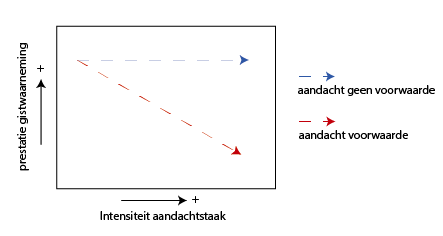
\includegraphics[width=1.0\linewidth]{illustratieHypothese.png}
\captionof{figure}{\color{Green} De visualisatie van onze hypothese: \'of aandacht een voorwaarde is voor bewustzijn wordt zichtbaar in de correlatie tussen gistperceptie en intensiteit van de aandachtstaak.}
\end{center}%\vspace{1cm}
%----------------------------------------------------------------------------------------
%   Methode
%----------------------------------------------------------------------------------------
\section*{Methode}
\textbf{Participanten} We hebben bij de selectie van proefpersonen (n=34) gestreefd naar een spreiding van leeftijd (mediaan=22, sd=15, range=17-60)en evenwichtige man/vrouw verhouding.(precies 1:1).\nocite{sporer2001recognizing} \\
\textbf{Materiaal} Het experiment is opgezet met behulp van PsychoPy2 software \cite{peirce2007psychopy, Peirce2009generating} en geanalyseerd met R \cite{Rsoftware}. De complete code inclusief alle foto's zijn te vinden op GitHub \cite{Grouls2017}.\\
\textbf{Stimuli} Gedurende 6 seconden steeds 2 tot 4 blauwe, ronde, bewegende objecten. De aandachtstaak van de proefpersonen was om te \textbf{tellen hoe vaak de objecten de rode lijn kruisten}. De bewustzijnstaak bestond uit het tegelijkertijd \textbf{waarnemen van afbeeldingen} met een mannen- of vrouwengezicht (zie Figuur 2). Het experiment werd voor elke conditie (2, 3 of 4 objecten) 20 keer herhaald met een mixed design (zie fig. 2).
\begin{center}\vspace{1cm}
		\captionof{figure}{Schematische weergave van het experiment.}
	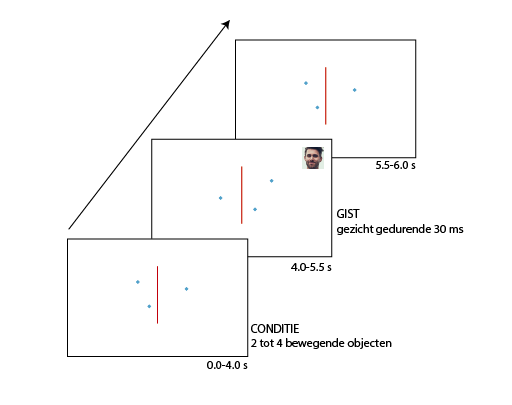
\includegraphics[width=0.8\linewidth]{Methode.png}

		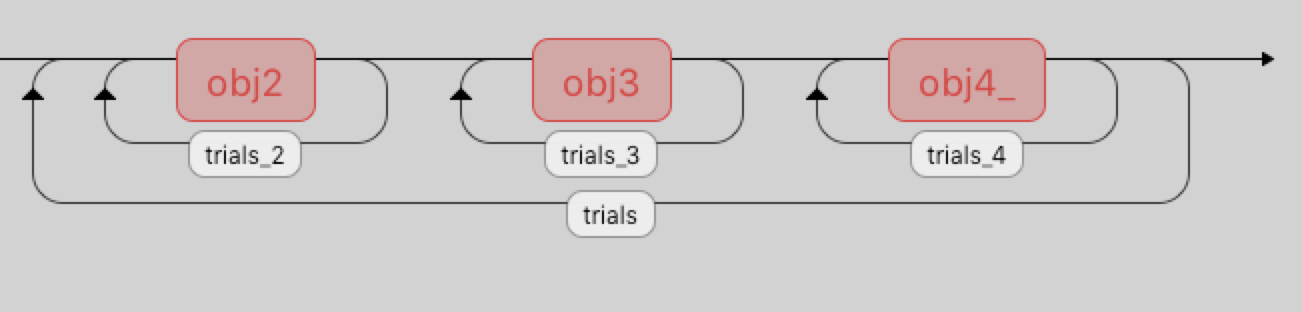
\includegraphics[width=0.8\linewidth]{opzetExperiment.png}
	\captionof{figure}{\color{Mixed design van de condities}
\end{center}
\section*{Resultaten}
\textbf{Prestatie objecttelling} Als de aandachtstaken inderdaad een textit{toenemende intesiviteit} hadden, dan moest \textbf{de prestatie op de objecttelling afnemen}. Dit is inderdaad het geval(zie tabel 1).
\begin{center}
	\captionof{table}{Prestatie correcte objecttelling (in \%)}
\begin{tabular}{c c c c c}
	 &  mean  & SDM & min & max\\
	\hline
	conditie 2 & 95.16 & 0.65 & 81.47 & 100.00\\
	conditie 3 & 93.94 & 0.87 & 79.91 & 99.58\\
	conditie 4 & 89.37 & 1.10 & 71.05 & 96.58\\
	\hline\\
\end{tabular}
\end{center}
\textbf{Trainings- en vermoeidheidseffecten} Wanneer we de ruwe data plotten voor prestatie op objecttelling, afgezet tegen het verloop in de tijd en differenti\"eren per conditie (fig. 4), valen twee dingen op:
\begin{enumerate}
	\item Alle lineaire regressies stijgen de eerste periode
	\item Na ongeveer 5 rondes (dus 15 experimenten) begint dit effect af te nemen en vermindert de score.
\end{enumerate}
 \begin{center}\vspace{1cm}
	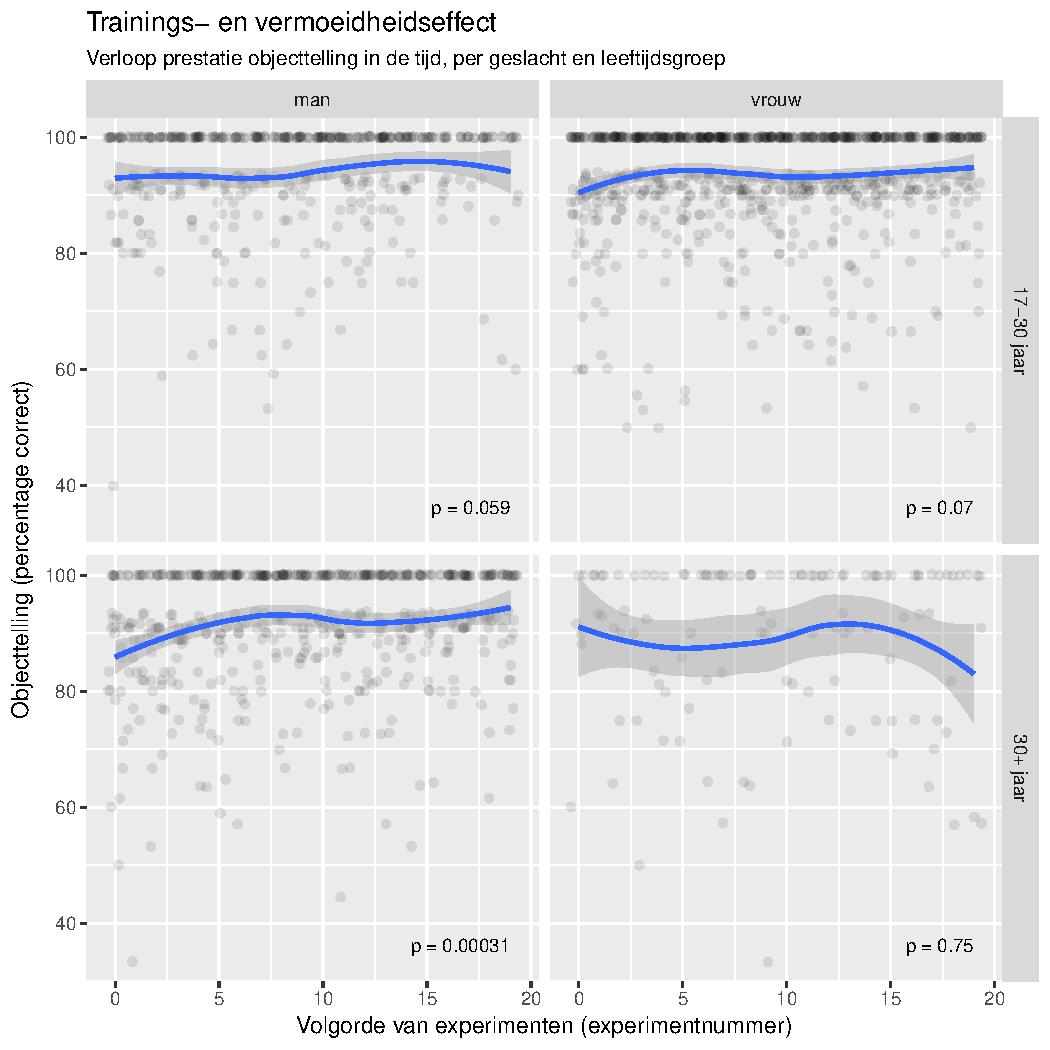
\includegraphics[width=0.8\linewidth]{training-grid.pdf}
	\captionof{figure}{\color{Green} De prestatie voor het correct tellen van de objecten uitgezet tegen het verloop in de tijd, uitgesplitst naar conditie.}
\end{center}\vspace{1cm}
Hoewel deze effecten invloed hebben op de modelvorming, was deze invloed niet significant. We bespreken dit verder in de discussie.\\\\
\textbf{Prestatie gistwaarneming} Wanneer we de prestatie op de gistwaarneming uitzetten tegen de conditie in een boxplot (zie fig. 5), zien we duidelijk dat voor de conditie met 4 objecten het percentage correcte gistwaarneming daalt. In tabel 2 is duidelijk af te lezen dat de verschillen tussen conditie 2 en 4 significant zijn. 
\begin{center}
\captionof{table}{Prestatie gistwaarneming (in \%)}
\begin{tabular}{c c c c c}
	 &  mean  & SDM & min & max\\
	\hline
	conditie 2 & 91.08 & 1.17 & 70 & 100\\
	conditie 3 & 91.32 & 1.51 & 70 & 100\\
	conditie 4 & 85.98 & 1.71 & 60 & 100\\
	\hline\\
\end{tabular}
\end{center}
Wanneer we op deze resultaten een lineaire regressie toepassen volgens $f(x)=a x+b$ is duidelijk zichtbaar dat dit een dalende lijn is (p = 0.017).
\begin{center}\vspace{1cm}
	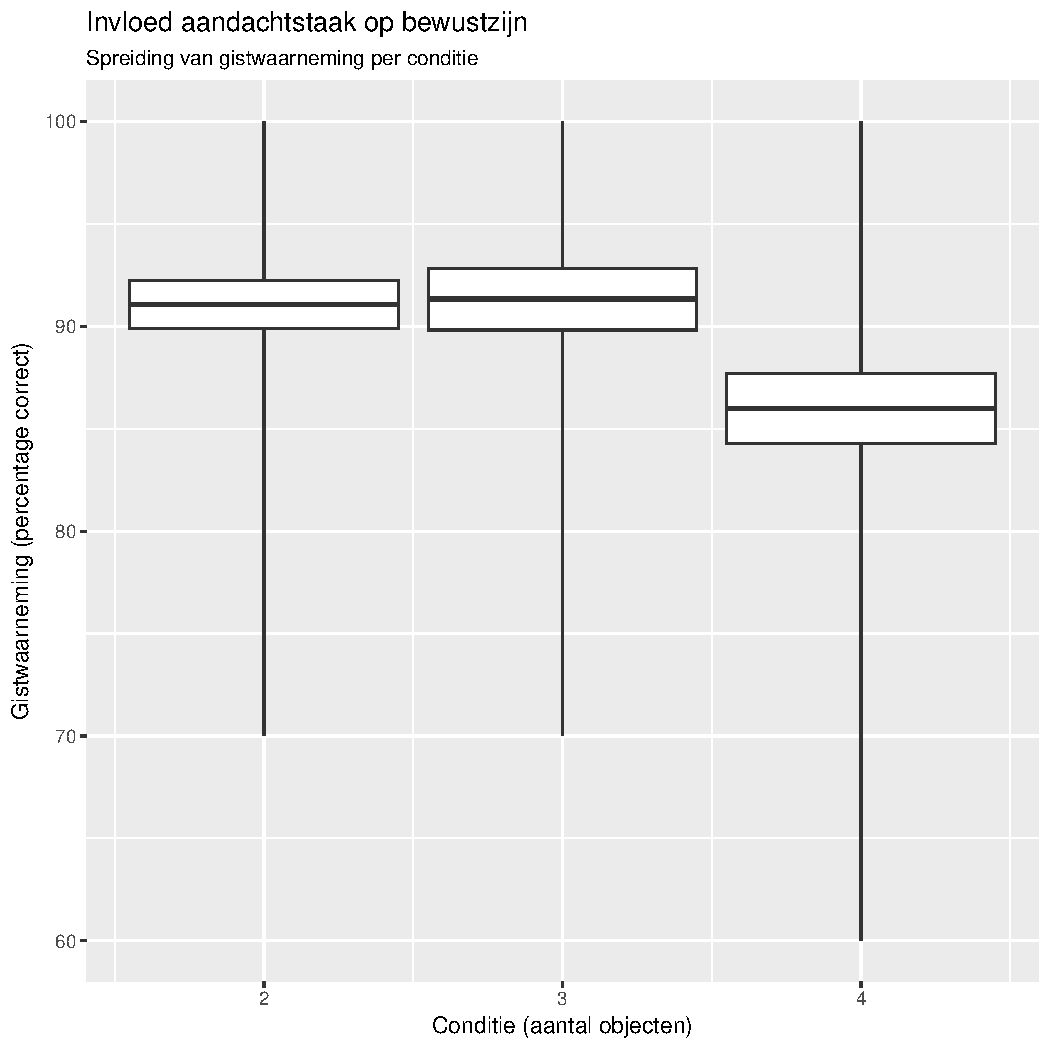
\includegraphics[width=0.8\linewidth]{boxplotGist-conditie.pdf}
	\captionof{figure}{\color{Green} Gistwaarneming per conditie. De errorbars geven de standaarddeviatie van het gemiddelde weer. De verticale lijn is de totale spreiding.}
\vspace{1cm}
	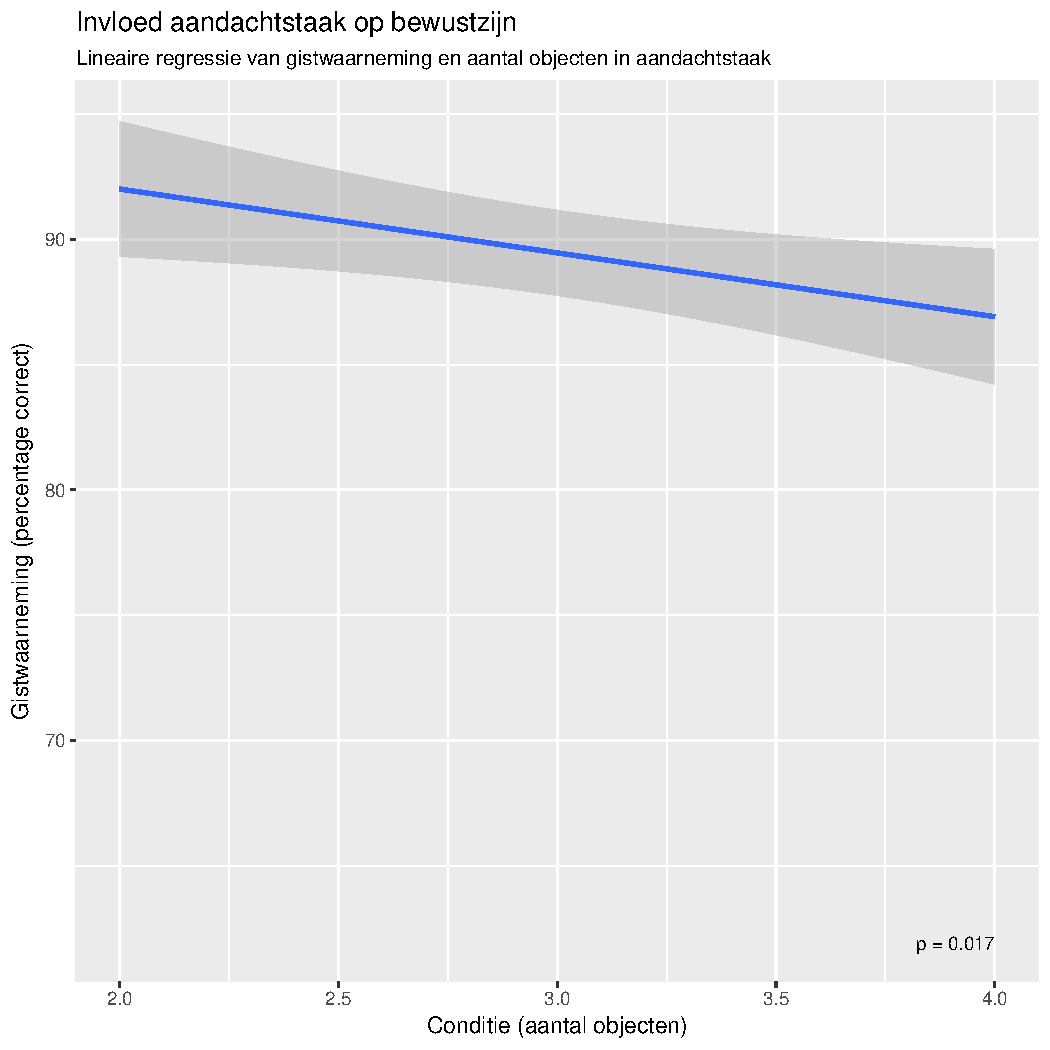
\includegraphics[width=0.8\linewidth]{lineaireRegressie.pdf}
	\captionof{figure}{\color{Green} De lineaire regressie volgens $f(x)=a x+b$}
\end{center}
De betrouwbaarheid van een lineair model is het hoogst, wanneer we het experiment ongeveer halverwege (p=0.007 na 9 rondes) zouden hebben afgekapt. Wij vermoeden dat dit effect veroorzaakt wordt door verschillen in trainings- en vermoeidheidseffecten.
\begin{center}
	\captionof{table}{invloed meegetelde rondes op modelvorming}
	\begin{tabular}{c c c}
		\hline
		p-waarde & $a$ & aantal rondes\\
		\hline
		0.007 & -0.035 & 9\\
		0.014 & -0.032 & 10\\
		0.043 & -0.024 & 15\\
		0.017 & -0.025 & 20\\
		\hline
	\end{tabular}
\end{center}
\subsection*{Discussie}
\begin{itemize}
\item Mannen van boven de 30 jaar blijken in onze data het \textbf{minst last te hebben van een vermoeidheidseffect} (zij worden het meest overtuigend steeds beter in het tellen van de objecten, p=0.00031) terwijl de prestatie van oudere juist afneemt.
\item Deze verschillen hebben \textbf{invloed op de betrouwbaarheid} van het lineaire model $f(x)=a x+b$, omdat de beschikbare aandacht na de 10e ronde sterk uiteen begon te lopen tussen proefpersonen onderling. 
\item Een mogelijk \textbf{verbeterpunt} van ons experiment is dan ook om het \textbf{op te knippen in twee delen}: 60x6 seconden balletjes tellen is voor sommige mensen gewoon te lang. 
\item Verder zijn er opvallende verschillen tussen mannen en vrouwen, die echter geen significant verschil maakten voor het eindresultaat (elke subgroep had een waarde van $a<0$).
\end{itemize}
\color{SaddleBrown} % SaddleBrown color for the conclusions to make them stand out
\section*{Conclusies}
\large Onze resultaten laten duidelijk zien dat de gistperceptie afneemt wanneer de aandacht verder wordt gemonopoliseerd. Ondanks dat wij dit zelf niet hadden verwacht, was het resultaat significant. Wij concluderen daarmee dat \textbf{aandacht een voorwaarde is voor bewustzijn}
\color{Black} % Set the color back to DarkSlateGray for the rest of the content









%----------------------------------------------------------------------------------------
%   CONCLUSIONS
%----------------------------------------------------------------------------------------


%----------------------------------------------------------------------------------------
%   FORTHCOMING RESEARCH
%----------------------------------------------------------------------------------------


 %----------------------------------------------------------------------------------------
%   REFERENCES
%----------------------------------------------------------------------------------------


%----------------------------------------------------------------------------------------
\bibliographystyle{apacite}
\bibliography{biblio}
\end{multicols}
\end{document}
              
            